\documentclass[12pt, oneside]{article}   	% use "amsart" instead of "article" for AMSLaTeX format
\usepackage{geometry}                		% See geometry.pdf to learn the layout options. There are lots.
\geometry{letterpaper}                   		% ... or a4paper or a5paper or ... 
%\geometry{landscape}                		% Activate for rotated page geometry
%\usepackage[parfill]{parskip}    		% Activate to begin paragraphs with an empty line rather than an indent
\usepackage{graphicx}				% Use pdf, png, jpg, or eps§ with pdflatex; use eps in DVI mode
								% TeX will automatically convert eps --> pdf in pdflatex		
\usepackage{amssymb}
\usepackage{amsmath}
\graphicspath{ {./images/} }

%SetFonts

%SetFonts


\title{Homework 1 - Supervised Learning Answers}
\author{Kasper Gammeltoft}
%\date{}							% Activate to display a given date or no date

\begin{document}
\maketitle

\section{1. Decision Trees}

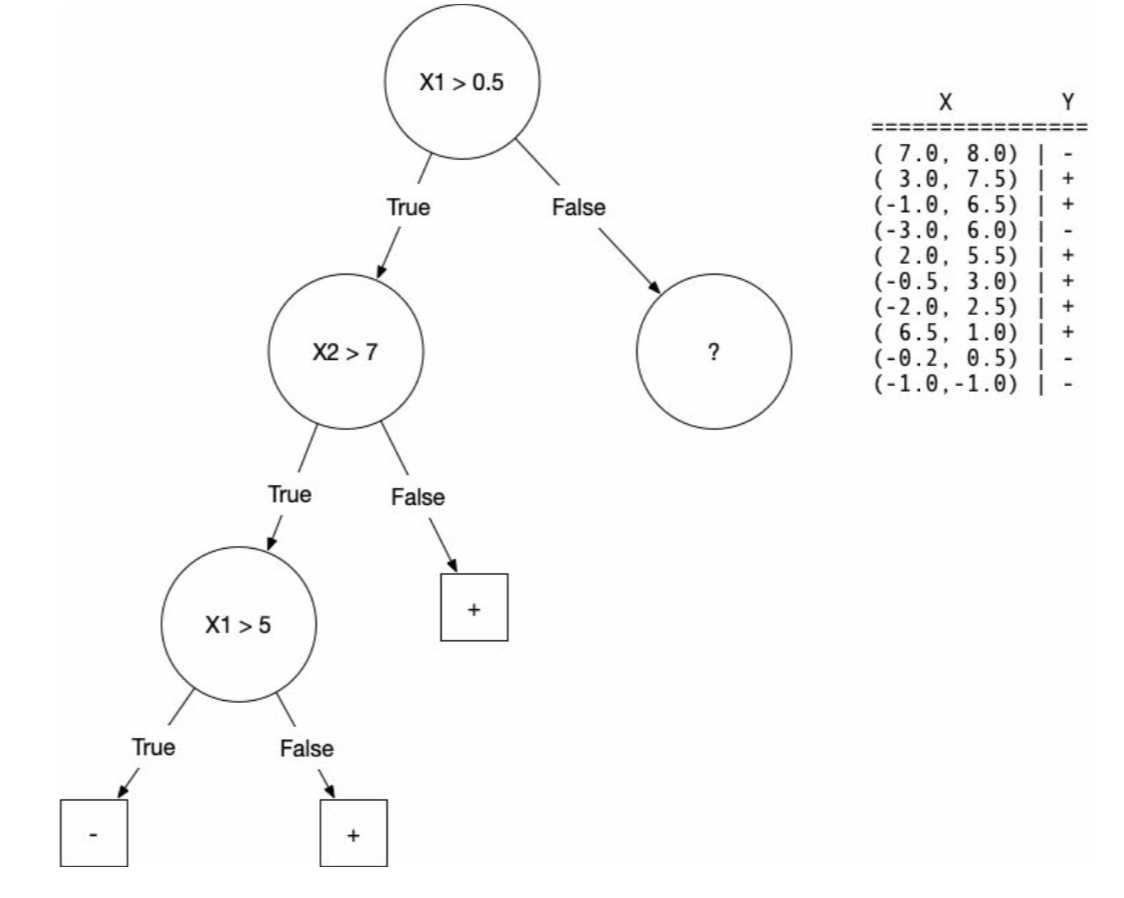
\includegraphics[scale=0.8]{decision_tree}

\subsection{}
Info gain with the three possible split choices.  Calculated by $H(D) - H(D|A)$ where\\ 
$$H(D) = \sum_{y\in D} -p(y_i) \cdot log_2(p(y_i))$$\\ \\
\begin{tabular}{c | c | c}
	$X2 > 6.5$ & $X2 > 0.5$ & $X2 > 0.0$ \\
	\hline
	$0$ & $1.57$ & $0.616$ \\
\end{tabular}

\subsection{}

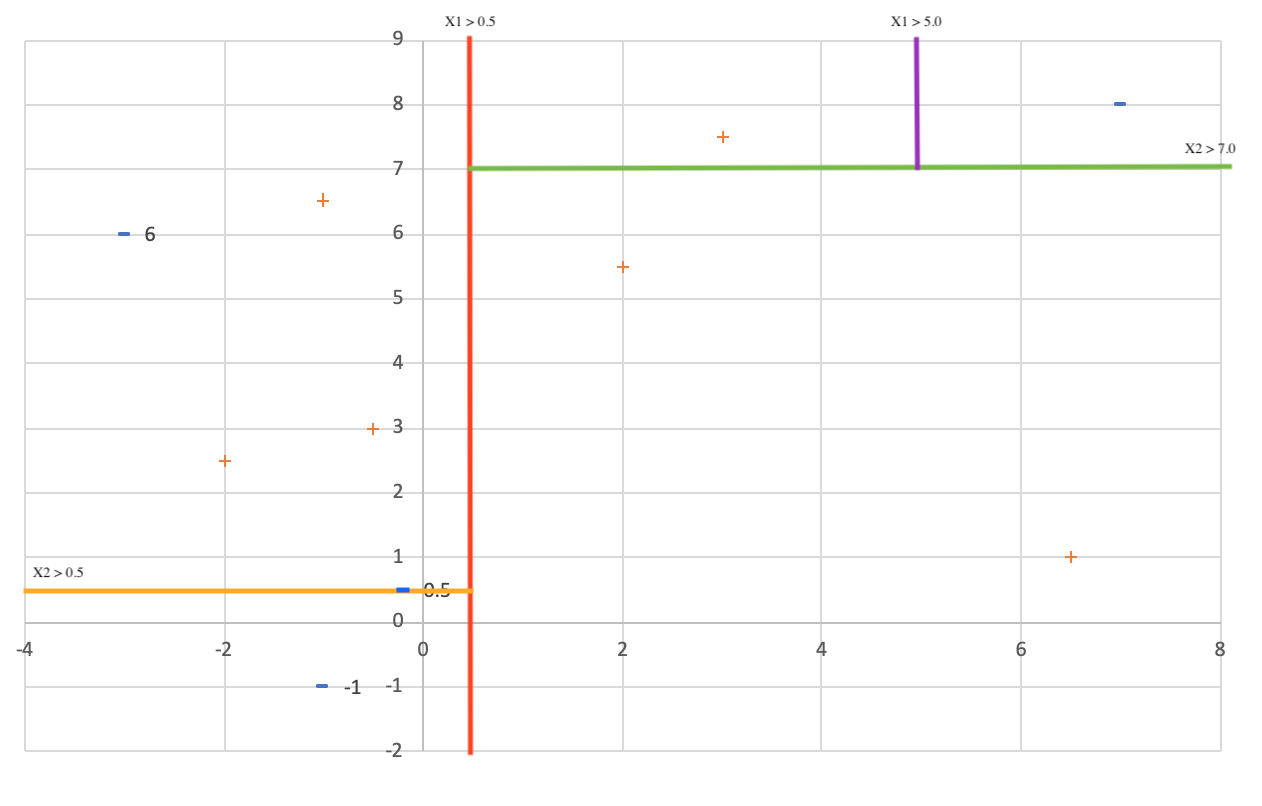
\includegraphics[scale=0.8]{decisionboundaryplot}

\subsection{}

Misclassification error for three possible split choices. \\ \\

\begin{tabular}{ c | c | c}
	$X2 > 6.5$ & $X2 > 0.5$ & $X2 > 0.0$ \\
	\hline
	$0.3$ & $0.1$ & $0.2$ \\ \\
\end{tabular} \\
The split with the largest info gain also has the smallest misclassification error, which is what was expected. As we gain more info per split, we expect less misclassification. 

\subsection{}

Another option is to consider the minimum and maximum points, then construct cuts for as many data points are along that range. For example, if we only have 3, 5, and 9, construct three possible splits: \\ \\
1. $\dfrac{9-3}{3} + 3 = 5$ \\
2. $\dfrac{9-3}{3} \cdot 2 + 3 = 7$ \\
3. $\dfrac{9-3}{3} \cdot 3 + 3 = 9$ \\ \\

We then pick the best split from these using the info gained. This does not yield a better result, however. As the data points we have are discrete, picking one of them is always the best policy- as it should be able to classify them just as well as any other point. 

\subsection{}

If we pick the split $X1>-3.0$, then we find we can perfectly classify the data using false as a - and true as a + leaf, after the previous $X2>0.5$ is true. 

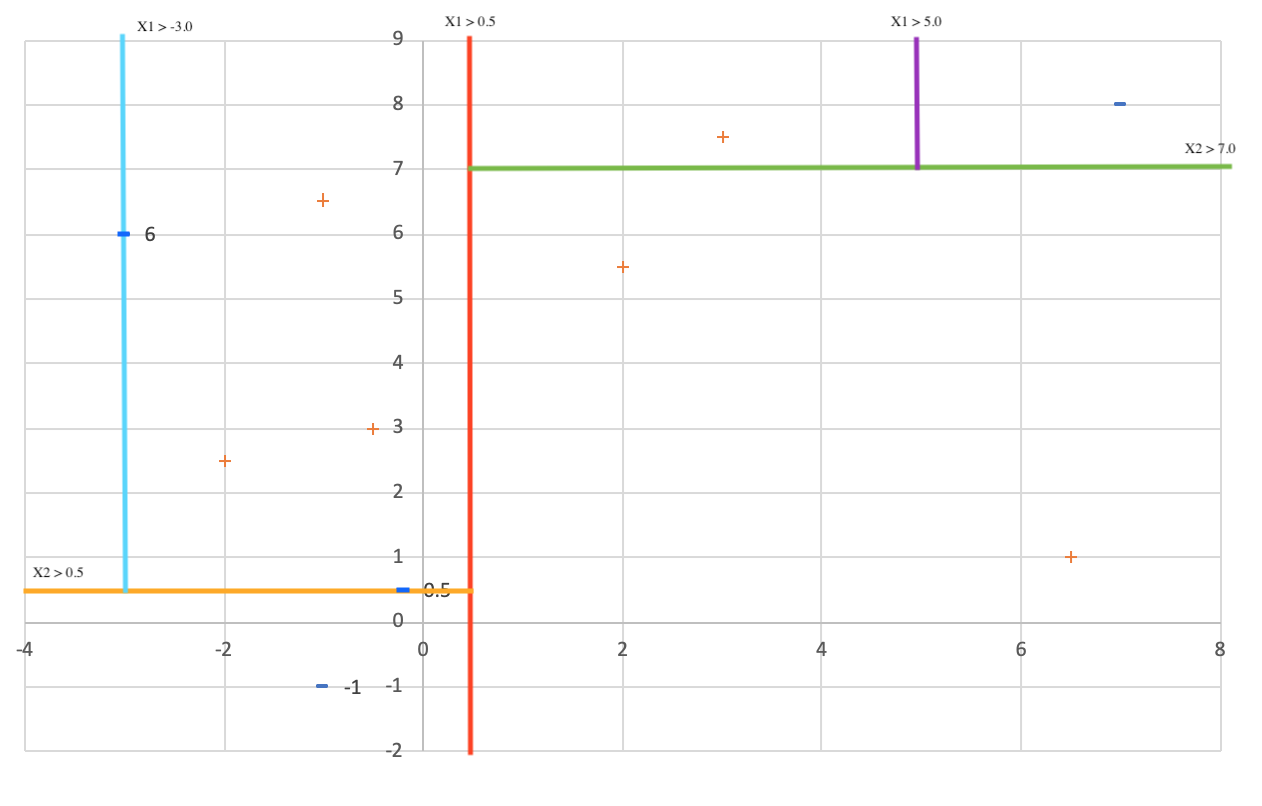
\includegraphics[scale=0.8]{decisionboundaryplot2}

\section{2. Polynomial Regression}

\subsection{}
There are exactly three ways to achieve features of power 2 with components $X_1$ and $X_2$: \\ \\
$X_1^2$, $X_2^2$, and $X_1X_2$. 

\subsection{}
To fit a polynomial of degree 2, we need all of the three features of degree two, plus those of degree one, plus those of degree 0. This would be something of the form: 
$$y = b_0 + b_1X_1 + b_2X_2 + b_3X_1^2 + b_4X_2^2 + b_5X_1X_2$$

This sums to be 6 features. 

\subsection{}

To generalize, we need to consider first how many features there are of degree $n$ given $X$ is in $d$ dimensions. This comes out to be $\binom{2n-1}{n-1} \cdot \binom{d}{n}$ as we can have only $n$ components from $X$ (if they have $degree >=1$ for each then any more than $n$ will be too many). We can also see we have $\binom{2n-1}{n-1}$ possibilities for each combination, as for $2$ we had $X_1^0X_2^2$, $X_1^1X_2^1$, and $X_1^2X_2^0$, as we count from 0 to 2. This is the multiset number with $n = n$ and $k = n$. Thus, if we need to generalize a polynomial of degree $p$, we can sum each possible number of features of degree 0 to $p$ given dimensionality $d$ of $X$. The number of features required is then given by:
$$ 1 + \sum_{i=1}^{p}{ \binom{2i-1}{i-1} \cdot \binom{d}{i}}$$

\section{3 Neural Networks}

\subsection{}

We are given the threshold function $g(x)$ and know that our weights are signified by $w^i_j$, specifying the $j^{th}$ weight of the $i^{th}$ layer. With this weight formation, we can only assume there is one perceptron per layer, or each perceptron will have the same weights for their inputs. Here we will assume each layer has $n$ nodes, and that $|x| = n$. Note that each perceptron has output $y = g(\sum_{j=1}^{n}w_j \cdot x_j)$, where $x_j$ is input from input layer or previous layer.\\ \\
$h(x)$ for the first layer would thus be $h_{1, j} = g(\sum_{j=1}^{n}x_jw^1_j)$. \\
$h(x)$ for the second layer would take this as an input: $h_{2, j} = g(\sum_{j=1}^{n}w^2_jh_{1, j})$. \\
Thus, plugging in $h_{1, j}$, we get $h(x) = g(\sum_{j=1}^{n}w^2_j \cdot g(\sum_{j=1}^{n}x_jw^1_j))$.

\subsection{}

Given the error function of means squared: $E(W, x, y) = 1/2{(y - h(x))}^2$, we can look at the partial derivative given a weight in either the first or second layer. Let's look at the second layer, with $j=1$: $w^2_1$. \\ \\
Plugging in our answer for $h(x)$ above, we get 
$$E(W, x, y) = 1/2{(y - g(\sum_{j=1}^{n}w^2_j \cdot g(\sum_{j=1}^{n}x_jw^1_j)))}^2$$
For simplicity, lets take the latter sum as a constant for now: $g(\sum_{j=1}^{n}x_jw^1_j)) = h_1$. Subbing this in and using the chain rule, we get 
$$E'(W,x,y) = -2(y - g(\sum_{j=1}^{n}w^2_j \cdot h_1)) \cdot g'(\sum_{j=1}^{n}w^2_j \cdot h_1) \cdot h_1$$
Assuming a 'nice' derivitive of $g$ allows this to be done rather easily, something important for neural networks. 

\section{4 K Nearest Neighbors}

\subsection{}

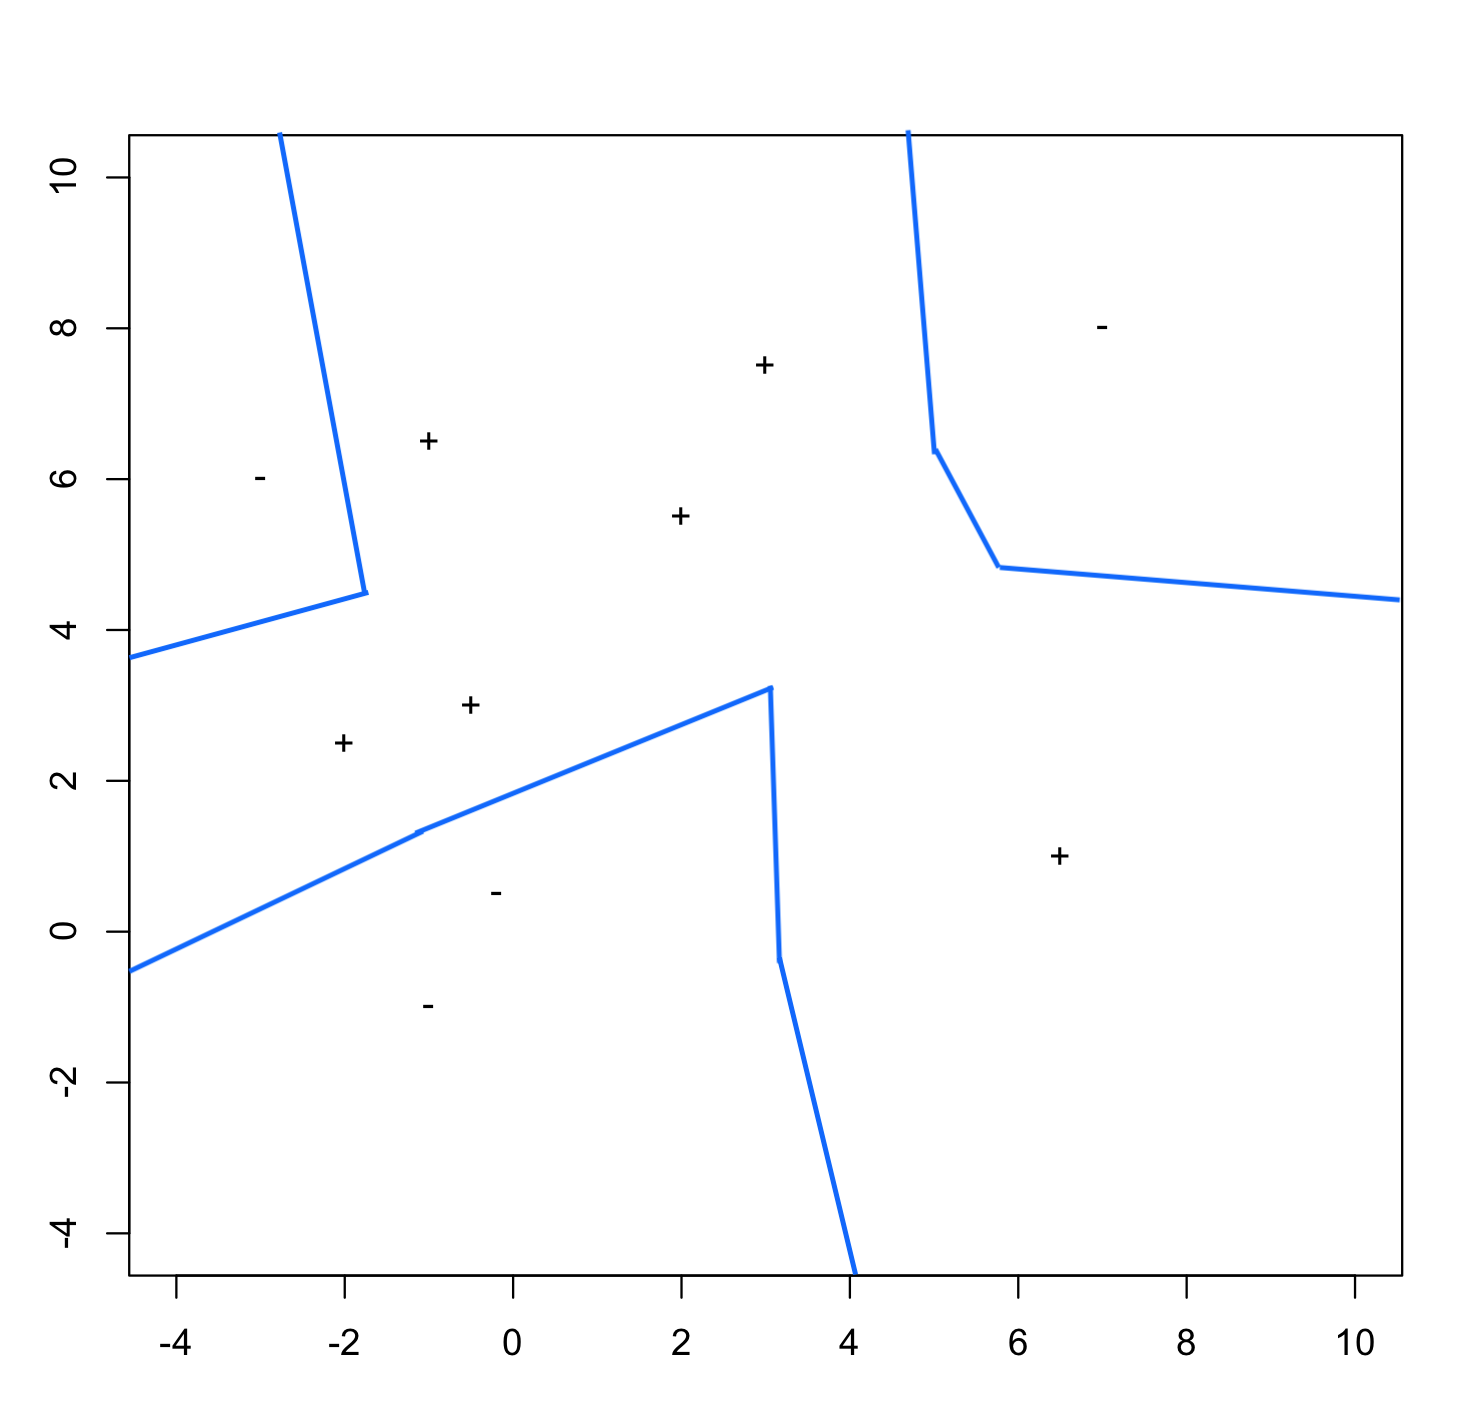
\includegraphics[scale=0.6]{approxDecisionBoundary}

\subsection{}

Misclassification error using leave one out: \\

\begin{tabular}{| c | c |}
	\hline
	$K$ & $Error$ \\
	\hline
	1 & 0.4\\
	\hline
	2 & 0.7\\
	\hline
	3 & 0.5\\
	\hline
	4 & 0.6\\
	\hline
	5 & 0.6\\ 
	\hline
\end{tabular}
\\

Clearly, $K=1$ is the best value for $K$, and has the least error.

\section{5 Ensemble Methods}

\subsection{}

Generally, bagging does not help with K-Nearest Neighbors. When $K=1$, all bagging will do is split the smaller $K=1$ learners amongst th data and average the results, effectively just setting $K$ to be a higher value. 

\subsection{}

Just as bagging, in effect, only increases the value of $K$, boosting will have the opposite effect. As we run the process many times and try to fit points we missed in the last iteration, it will give more weight to those points. This will have the same effect as decreasing $K$. 

\end{document} 